% !Mode:: "TeX:UTF-8"	% read in as utf8 file.

\chapter{Strain}

The deformation of a thin straight rod into a closed loop. The length of the rod remains almost unchanged during the deformation, which indicates that the strain is small. In this particular case of bending, displacements associated with rigid translations and rotations of material elements in the rod are much greater than displacements associated with straining.

\begin{figure}[h]
	\centering
	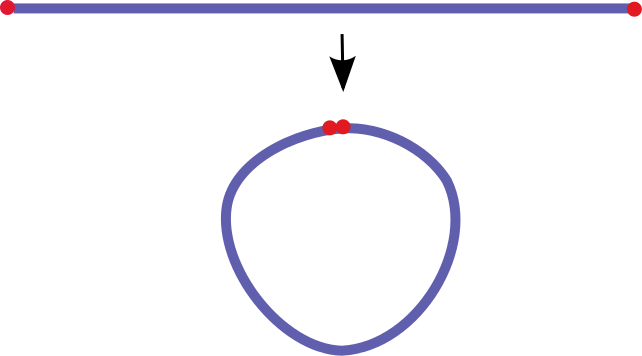
\includegraphics[width=0.7\linewidth]{figure/DeformationOfRod.png}
	\caption{deformation of rod}
	\label{fig:DeformationOfRod}
\end{figure}

\section{Preliminary Definitions}
\begin{itemize}
	\item displacement - the total movement of a point with respect to a fixed reference coordinates is called \textit{displacement}
	\item Deformation - the relative movement of a point with respect to another point on the body is called \textit{deformation}
	\item Lagrangian Strain - \textit{Lagrangian Strain} is computed from deformation by using the original undeformed geometry as the reference geometry
	\item Eulerian Strain - \textit{Eulerian Strain} is computed from deformation by using the final deformed geometry as the reference geometry.
	\item Deflection - a term to describe the magnitude to which a structural element is displaced when subject to an applied load.
\end{itemize}

\section{Average Normal Strain}
\begin{figure}[h]
\centering
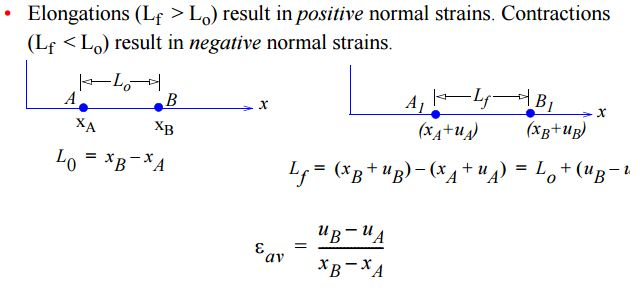
\includegraphics[width=0.7\linewidth]{figure/average_normal_strain}
\caption{Average normal strain}
\label{fig:strain_def}
\end{figure}

\section{Strain components}
%\begin{figure}[h]
%\centering
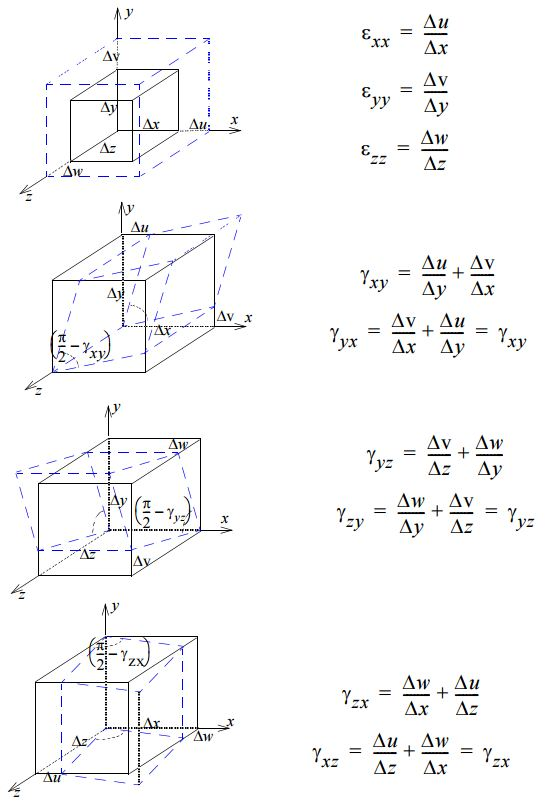
\includegraphics[width=0.7\linewidth]{figure/strain_components}
\captionof{figure}{strain components}
\label{fig:strain_components}
%\end{figure}

\section{Engineering Strain}
\begin{itemize}
\item Engineering strain matrix:
\begin{equation*}
\begin{bmatrix}
\varepsilon_{xx} & \gamma_{xy} & \gamma_{xz} \\
\gamma_{yx} & \varepsilon_{yy} & \gamma_{yz} \\
\gamma_{zx} & \gamma_{zy} & \varepsilon_{zz}
\end{bmatrix}
\end{equation*}
\item Plane strain matrix:
\begin{equation*}
\begin{bmatrix}
\varepsilon_{xx} & \gamma_{xy} & 0 \\
\gamma_{yx} & \varepsilon_{yy} & 0 \\
0 & 0 & 0
\end{bmatrix}
\end{equation*}
\item Strain at a point
\begin{align*}
\varepsilon_{xx} &= \lim_{\Delta x \to 0} \left( \dfrac{\Delta u}{\Delta x} = \dfrac{\partial u}{\partial x}\right)\\
\varepsilon_{yy} &= \dfrac{\partial v}{\partial y} \\
\varepsilon_{zz} &= \dfrac{\partial w}{\partial z} \\
\gamma_{xy} &= \gamma_{yx} = \lim_{\substack{\Delta x\to 0 \\ \Delta y\to 0}} \left( \dfrac{\Delta u}{\Delta y}+\dfrac{\Delta v}{\Delta x}\right) = \dfrac{\partial u}{\partial y} + \dfrac{\partial v}{\partial x} \\
\gamma_{yz} &= \gamma_{zy} = \dfrac{\partial v}{\partial z} + \dfrac{\partial w}{\partial y} \\
\gamma_{zx} &= \gamma_{xz} = \dfrac{\partial w}{\partial x} + \dfrac{\partial u}{\partial z}
\end{align*}
\end{itemize}

\section{linearized Cauchy strain}
Our technique uses linearized Cauchy strain and stiffness warping to avoid linearization artifacts for large deformations.

The elastic energy density of a deformable body is defined in terms of \textbf{stress} and \textbf{strain} within the object. For the latter, we employ the linear Cauchy strain $ \epsilon $, which depends on the Jacobian $ \Delta \mathbf{u} $ of the deformation field $ \mathbf{u} $:

\begin{equation}
\mathbf{\epsilon} = \dfrac{1}{2} (\Delta \mathbf{u} + \Delta \mathbf{u}^\mathit{T})
\label{Eq: constitutive relation}
\end{equation}

The strain of the material in turn causes internal forces, represented by the $ 3\times 3 $ stress matrix $ \sigma $. We assume a \textbf{Hookean material}, i.e., a linear stress-strain relation. Note that $ \epsilon $ and $ \sigma $ both are $ 3\times 3 $ matrices.

Representing the stress by a 6D vector as well reduces the constitutive relation \ref{Eq: constitutive relation} to a simple $ 6\times 6 $ matrix product:

\begin{equation}
\sigma = \mathbf{C}\epsilon
\end{equation}

where the \textbf{constitutive matrix} $ \mathbf{C} $ only depends on the material' elasticity modulus and Poisson ratio, controlling stiffness and volume preservation.

With stress and strain defined at any material point $ \mathbf{x} $, the total elastic energy $ \mathit{U}(\mathbf{u}) $ can finally be computed as the integral of stress times strain over the object's volume:

\begin{equation}
U(\mathbf{u}) = \dfrac{1}{2}\int_v{\mathbf{\sigma}^T \mathbf{\epsilon}} = \dfrac{1}{2}\int_V{\mathbf{\epsilon}^T \mathbf{C} \mathbf{\epsilon}}
\label{Eq: continuum energy function}
\end{equation}

\section{Discretize energy function}
In order to discretize the energy function \ref{Eq: continuum energy function} the continuum object is decomposed into a finite number of elements, and each node $ i\in {1, \ldots, n} $ of this decomposition is associated wit a material position $ \mathbf{x}_i $, a displacement value $ \mathbf{u}_i= \mathbf{u}(\mathbf{x}_i) $, and a scalar shape function $ \Phi_i(\mathbf{x}) $. With this, the continuous function $ \mathbf{u} (\mathbf{x}) $ can be approximated by:

\begin{equation}
\mathbf{u}(\mathbf{x}) = \sum_{i=1}^{n}{\mathbf{u}_i\Phi_i(\mathbf{x})}
\end{equation}

While graphics applications typically employ \textbf{tetrahedron} or \textbf{hexahedral} decomposition, our goal is to find an FEM formulation for \textbf{convex polyhedron}. This requires interpolation function $ \Phi_i $ for convex polyhedra that are suitable for FEM computation.